%Version 3 October 2023
%DIF LATEXDIFF DIFFERENCE FILE
%DIF DEL manuscript_long_version/sn-article-template/sn-article.tex   Fri Apr 26 18:04:00 2024
%DIF ADD manuscript/sn-article.tex                                    Fri May  3 10:47:00 2024
% See section 11 of the User Manual for version history
%
%%%%%%%%%%%%%%%%%%%%%%%%%%%%%%%%%%%%%%%%%%%%%%%%%%%%%%%%%%%%%%%%%%%%%%
%%                                                                 %%
%% Please do not use \input{...} to include other tex files.       %%
%% Submit your LaTeX manuscript as one .tex document.              %%
%%                                                                 %%
%% All additional figures and files should be attached             %%
%% separately and not embedded in the \TeX\ document itself.       %%
%%                                                                 %%
%%%%%%%%%%%%%%%%%%%%%%%%%%%%%%%%%%%%%%%%%%%%%%%%%%%%%%%%%%%%%%%%%%%%%

%%\documentclass[referee,sn-basic]{sn-jnl}% referee option is meant for double line spacing

%%=======================================================%%
%% to print line numbers in the margin use lineno option %%
%%=======================================================%%

\documentclass[lineno,sn-basic]{sn-jnl}% Basic Springer Nature Reference Style/Chemistry Reference Style

%%======================================================%%
%% to compile with pdflatex/xelatex use pdflatex option %%
%%======================================================%%

%%\documentclass[pdflatex,sn-basic]{sn-jnl}% Basic Springer Nature Reference Style/Chemistry Reference Style


%%Note: the following reference styles support Namedate and Numbered referencing. By default the style follows the most common style. To switch between the options you can add or remove “Numbered” in the optional parenthesis. 
%%The option is available for: sn-basic.bst, sn-vancouver.bst, sn-chicago.bst%  
 
%%\documentclass[sn-nature]{sn-jnl}% Style for submissions to Nature Portfolio journals
%%\documentclass[sn-basic]{sn-jnl}% Basic Springer Nature Reference Style/Chemistry Reference Style
% \documentclass[sn-mathphys-num]{sn-jnl}% Math and Physical Sciences Numbered Reference Style 
%%\documentclass[sn-mathphys-ay]{sn-jnl}% Math and Physical Sciences Author Year Reference Style
%%\documentclass[sn-aps]{sn-jnl}% American Physical Society (APS) Reference Style
%%\documentclass[sn-vancouver,Numbered]{sn-jnl}% Vancouver Reference Style
%%\documentclass[sn-apa]{sn-jnl}% APA Reference Style 
%%\documentclass[sn-chicago]{sn-jnl}% Chicago-based Humanities Reference Style

%%%% Standard Packages
%%<additional latex packages if required can be included here>

\usepackage{graphicx}%
\usepackage{multirow}%
\usepackage{amsmath,amssymb,amsfonts}%
\usepackage{amsthm}%
\usepackage{mathrsfs}%
\usepackage[title]{appendix}%
\usepackage{xcolor}%
\usepackage{textcomp}%
\usepackage{manyfoot}%
\usepackage{booktabs}%
\usepackage{algorithm}%
\usepackage{algorithmicx}%
\usepackage{algpseudocode}%
\usepackage{listings}%
% \usepackage{natbib}%

\raggedbottom
%%\unnumbered% uncomment this for unnumbered level heads
%DIF PREAMBLE EXTENSION ADDED BY LATEXDIFF
%DIF UNDERLINE PREAMBLE %DIF PREAMBLE
\RequirePackage[normalem]{ulem} %DIF PREAMBLE
\RequirePackage{color}\definecolor{RED}{rgb}{1,0,0}\definecolor{BLUE}{rgb}{0,0,1} %DIF PREAMBLE
\providecommand{\DIFadd}[1]{{\protect\color{blue}\uwave{#1}}} %DIF PREAMBLE
\providecommand{\DIFdel}[1]{{\protect\color{red}\sout{#1}}}                      %DIF PREAMBLE
%DIF SAFE PREAMBLE %DIF PREAMBLE
\providecommand{\DIFaddbegin}{} %DIF PREAMBLE
\providecommand{\DIFaddend}{} %DIF PREAMBLE
\providecommand{\DIFdelbegin}{} %DIF PREAMBLE
\providecommand{\DIFdelend}{} %DIF PREAMBLE
\providecommand{\DIFmodbegin}{} %DIF PREAMBLE
\providecommand{\DIFmodend}{} %DIF PREAMBLE
%DIF FLOATSAFE PREAMBLE %DIF PREAMBLE
\providecommand{\DIFaddFL}[1]{\DIFadd{#1}} %DIF PREAMBLE
\providecommand{\DIFdelFL}[1]{\DIFdel{#1}} %DIF PREAMBLE
\providecommand{\DIFaddbeginFL}{} %DIF PREAMBLE
\providecommand{\DIFaddendFL}{} %DIF PREAMBLE
\providecommand{\DIFdelbeginFL}{} %DIF PREAMBLE
\providecommand{\DIFdelendFL}{} %DIF PREAMBLE
\newcommand{\DIFscaledelfig}{0.5}
%DIF HIGHLIGHTGRAPHICS PREAMBLE %DIF PREAMBLE
\RequirePackage{settobox} %DIF PREAMBLE
\RequirePackage{letltxmacro} %DIF PREAMBLE
\newsavebox{\DIFdelgraphicsbox} %DIF PREAMBLE
\newlength{\DIFdelgraphicswidth} %DIF PREAMBLE
\newlength{\DIFdelgraphicsheight} %DIF PREAMBLE
% store original definition of \includegraphics %DIF PREAMBLE
\LetLtxMacro{\DIFOincludegraphics}{\includegraphics} %DIF PREAMBLE
\newcommand{\DIFaddincludegraphics}[2][]{{\color{blue}\fbox{\DIFOincludegraphics[#1]{#2}}}} %DIF PREAMBLE
\newcommand{\DIFdelincludegraphics}[2][]{% %DIF PREAMBLE
\sbox{\DIFdelgraphicsbox}{\DIFOincludegraphics[#1]{#2}}% %DIF PREAMBLE
\settoboxwidth{\DIFdelgraphicswidth}{\DIFdelgraphicsbox} %DIF PREAMBLE
\settoboxtotalheight{\DIFdelgraphicsheight}{\DIFdelgraphicsbox} %DIF PREAMBLE
\scalebox{\DIFscaledelfig}{% %DIF PREAMBLE
\parbox[b]{\DIFdelgraphicswidth}{\usebox{\DIFdelgraphicsbox}\\[-\baselineskip] \rule{\DIFdelgraphicswidth}{0em}}\llap{\resizebox{\DIFdelgraphicswidth}{\DIFdelgraphicsheight}{% %DIF PREAMBLE
\setlength{\unitlength}{\DIFdelgraphicswidth}% %DIF PREAMBLE
\begin{picture}(1,1)% %DIF PREAMBLE
\thicklines\linethickness{2pt} %DIF PREAMBLE
{\color[rgb]{1,0,0}\put(0,0){\framebox(1,1){}}}% %DIF PREAMBLE
{\color[rgb]{1,0,0}\put(0,0){\line( 1,1){1}}}% %DIF PREAMBLE
{\color[rgb]{1,0,0}\put(0,1){\line(1,-1){1}}}% %DIF PREAMBLE
\end{picture}% %DIF PREAMBLE
}\hspace*{3pt}}} %DIF PREAMBLE
} %DIF PREAMBLE
\LetLtxMacro{\DIFOaddbegin}{\DIFaddbegin} %DIF PREAMBLE
\LetLtxMacro{\DIFOaddend}{\DIFaddend} %DIF PREAMBLE
\LetLtxMacro{\DIFOdelbegin}{\DIFdelbegin} %DIF PREAMBLE
\LetLtxMacro{\DIFOdelend}{\DIFdelend} %DIF PREAMBLE
\DeclareRobustCommand{\DIFaddbegin}{\DIFOaddbegin \let\includegraphics\DIFaddincludegraphics} %DIF PREAMBLE
\DeclareRobustCommand{\DIFaddend}{\DIFOaddend \let\includegraphics\DIFOincludegraphics} %DIF PREAMBLE
\DeclareRobustCommand{\DIFdelbegin}{\DIFOdelbegin \let\includegraphics\DIFdelincludegraphics} %DIF PREAMBLE
\DeclareRobustCommand{\DIFdelend}{\DIFOaddend \let\includegraphics\DIFOincludegraphics} %DIF PREAMBLE
\LetLtxMacro{\DIFOaddbeginFL}{\DIFaddbeginFL} %DIF PREAMBLE
\LetLtxMacro{\DIFOaddendFL}{\DIFaddendFL} %DIF PREAMBLE
\LetLtxMacro{\DIFOdelbeginFL}{\DIFdelbeginFL} %DIF PREAMBLE
\LetLtxMacro{\DIFOdelendFL}{\DIFdelendFL} %DIF PREAMBLE
\DeclareRobustCommand{\DIFaddbeginFL}{\DIFOaddbeginFL \let\includegraphics\DIFaddincludegraphics} %DIF PREAMBLE
\DeclareRobustCommand{\DIFaddendFL}{\DIFOaddendFL \let\includegraphics\DIFOincludegraphics} %DIF PREAMBLE
\DeclareRobustCommand{\DIFdelbeginFL}{\DIFOdelbeginFL \let\includegraphics\DIFdelincludegraphics} %DIF PREAMBLE
\DeclareRobustCommand{\DIFdelendFL}{\DIFOaddendFL \let\includegraphics\DIFOincludegraphics} %DIF PREAMBLE
%DIF COLORLISTINGS PREAMBLE %DIF PREAMBLE
\RequirePackage{listings} %DIF PREAMBLE
\RequirePackage{color} %DIF PREAMBLE
\lstdefinelanguage{DIFcode}{ %DIF PREAMBLE
%DIF DIFCODE_UNDERLINE %DIF PREAMBLE
  moredelim=[il][\color{red}\sout]{\%DIF\ <\ }, %DIF PREAMBLE
  moredelim=[il][\color{blue}\uwave]{\%DIF\ >\ } %DIF PREAMBLE
} %DIF PREAMBLE
\lstdefinestyle{DIFverbatimstyle}{ %DIF PREAMBLE
	language=DIFcode, %DIF PREAMBLE
	basicstyle=\ttfamily, %DIF PREAMBLE
	columns=fullflexible, %DIF PREAMBLE
	keepspaces=true %DIF PREAMBLE
} %DIF PREAMBLE
\lstnewenvironment{DIFverbatim}{\lstset{style=DIFverbatimstyle}}{} %DIF PREAMBLE
\lstnewenvironment{DIFverbatim*}{\lstset{style=DIFverbatimstyle,showspaces=true}}{} %DIF PREAMBLE
%DIF END PREAMBLE EXTENSION ADDED BY LATEXDIFF

\begin{document}

% \title[Article Title]{Does the presence of leads in the Arctic sea ice have an impact on the ocean?}

\title[Article Title]{Is the surface forcing in sea ice leads transferred to the Arctic ocean interior?}
%%=============================================================%%
%% GivenName	-> \fnm{Joergen W.}
%% Particle	-> \spfx{van der} -> surname prefix
%% FamilyName	-> \sur{Ploeg}
%% Suffix	-> \sfx{IV}
%% \author*[1,2]{\fnm{Joergen W.} \spfx{van der} \sur{Ploeg} 
%%  \sfx{IV}}\email{iauthor@gmail.com}
%%=============================================================%%

\author*[1]{\fnm{Josu\'e} \sur{Mart\'inez-Moreno}}\email{josue.martinez.moreno@ifremer.fr}

\author[1]{\fnm{Camille} \sur{Lique}}\email{camille.lique@ifremer.fr}
%\equalcont{These authors contributed equally to this work.}

\author[1]{\fnm{Claude} \sur{Talandier}}\email{claude.Talandier@ifremer.fr}
%\equalcont{These authors contributed equally to this work.}

\affil*[1]{\orgdiv{Univ Brest, CNRS, Ifremer, IRD }, \orgname{Laboratoire d'Oc\'eanographie Physique et Spatiale (LOPS)}, \orgaddress{Institut Universitaire Européen de la Mer, \city{Plouzan\'e}, \postcode{F29280}, \state{Bretagne}, \country{France}}}


%%==================================%%
%% Sample for unstructured abstract %%
%%==================================%%

\DIFdelbegin %DIFDELCMD < \abstract{The Arctic sea-ice, in particular the ice-pack, acts as an insulator between the atmosphere and the ocean below. Leads, common in Arctic sea ice, facilitate exchanges of heat, salt, moisture and gases between the ocean and the atmosphere. Therefore, leads can influence heat exchanges, ice melt or growth, ocean dynamics, and the atmospheric boundary layer. The existing literature suggests that leads play a significant role in the heat budget of the surface of the ocean and likely impact water mass transformation within the Arctic. However, due to the lack of observations and high resolution models capable to resolve leads, an estimate of the impact of leads in the ocean buoyancy has been elusive.  Here, we explore the magnitude and impact in the ocean surface caused by the leads using SEDNA, a subkilometer pan-Arctic hindcast (1/60$^\circ$; NEMO model). Leads account for 22\% of the sea-ice cover extent, and within them, there is approximately 25\% of the total surface water mass transformation. 
%DIFDELCMD < The buoyancy flux and water mass transformation in leads are similar to those underneath the surrounding ice covered oceans and the percentage of water mass transformation through leads matches their area coverage. 
%DIFDELCMD < Thus, the present estimate indicates that leads have a small contribution to Arctic Ocean dynamics, contrary to previous hypotheses.}
%DIFDELCMD < %%%
\DIFdelend \DIFaddbegin \abstract{The Arctic sea-ice, in particular the ice-pack, acts as an insulator between the atmosphere and the ocean below. Leads, common in Arctic sea ice, facilitate exchanges of heat, salt, moisture and gases between the ocean and the atmosphere. Existing literature suggests that leads play a significant role in the heat budget of the surface of the ocean and likely impact water mass transformation within the Arctic. However, due to the lack of observations and high resolution models capable to resolve leads, an estimate of the impact of leads in the ocean buoyancy has been elusive.  Here, we explore the magnitude and impact in the ocean surface caused by the leads using SEDNA, a subkilometer pan-Arctic hindcast (1/60$^\circ$; NEMO model). Leads account for 22\% of the sea-ice cover extent, and within them, there is approximately 25\% of the total surface water mass transformation. 
The buoyancy flux and water mass transformation in leads are similar to those underneath the surrounding ice covered oceans and the percentage of water mass transformation through leads matches their area coverage. 
Thus, the present estimate indicates that leads have a small contribution to Arctic Ocean dynamics, contrary to previous hypotheses.}
\DIFaddend 

\keywords{Arctic, Leads, Buoyancy flux}

%%\pacs[JEL Classification]{D8, H51}
%%\pacs[MSC Classification]{35A01, 65L10, 65L12, 65L20, 65L70}

\maketitle

\DIFdelbegin \section{\DIFdel{Introduction}}%DIFAUXCMD
\addtocounter{section}{-1}%DIFAUXCMD
%DIFDELCMD < \label{sec1}
%DIFDELCMD < %%%
\DIFdelend %DIF > \section{Introduction}\label{sec1}

The Arctic sea-ice \DIFdelbegin \DIFdel{plays a crucial role in regulating }\DIFdelend \DIFaddbegin \DIFadd{regulates }\DIFaddend Earth's climate by acting as a natural insulator between the atmosphere and the ocean\DIFdelbegin \DIFdel{below}\DIFdelend . This insulating property acts as a thermal barrier, limiting heat loss from the ocean to the atmosphere and minimizing evaporation \citep{Wettlaufer_insulator_1997, Untersteiner_ice_insulator_1961}. An ubiquitous feature of Arctic sea ice is the formation and persistence of leads. Leads occur across the polar oceans, both in the marginal ice zone (MIZ; $15-80\%$ sea ice concentration) and the ice pack ($>80\%$ sea ice concentration). \DIFdelbegin \DIFdel{The difference between leads in these two regions arise from the mechanism driving their formation. }\DIFdelend Within the MIZ, leads are primarily formed by advection of sea ice, while in the ice pack, leads form through deformation of the sea ice (\DIFdelbegin \DIFdel{ice pack leads are }\DIFdelend commonly known in literature as ``linear kinematic features"; LKFs). 
The main forcing of the sea ice advection and deformation \DIFdelbegin \DIFdel{, thus the formation of leads, }\DIFdelend is the wind \citep{Linow_lkf_2017, Hutter_scaling_lkf_2018}, with a smaller contribution \DIFdelbegin \DIFdel{by the }\DIFdelend \DIFaddbegin \DIFadd{from }\DIFaddend ocean currents \citep{Willmes_leads_currents_2023}.
Leads can result in an opening \DIFdelbegin \DIFdel{within }\DIFdelend \DIFaddbegin \DIFadd{of }\DIFaddend the sea ice cover \citep{Rampal_nextsim_2016, Hutchings_model_lkf_2005, Richter_pack_stress_2002} with spatial scales of \DIFdelbegin \DIFdel{a few }\DIFdelend meters to kilometers in width and a few kilometers up to hundreds of kilometers in length, and temporal scales ranging from a few hours up to a few days \citep{Linow_lkf_2017, Wernecke_Lead_2015, Tschudi_obs_leads_1998}. Thus, they \DIFdelbegin \DIFdel{are windows between the ocean and the atmosphere that can allow large flux exchanges, and }\DIFdelend \DIFaddbegin \DIFadd{can }\DIFaddend locally impact the surface forcing \DIFdelbegin \DIFdel{of }\DIFdelend \DIFaddbegin \DIFadd{in }\DIFaddend the ice covered polar oceans \citep{Lupkes_leads_2008}.

Once leads are formed, atmospheric forcing in conjunction with localized upwelling or downwelling occuring in the surface layer can result in important heat fluxes at the ocean surface ($\mathcal{O} \sim 100 W/m^2$; \citealp{Bourgault_flux_lkf_2020,McPhee_LKF_2005,Marcq_flux_lead_2012,Maykut_heat_1986}), instigating localized melting or freezing of sea ice \citep{Albedyll_thickness_dis_2022}. For example, \citet{Boutin_rheology_2023} estimated that 35\% of the total sea ice growth during winter occurs within the leads in the ice pack. The Arctic ice covered ocean is a $\beta$-ocean, i.e. the ocean stratification is mainly controlled by salinity\DIFdelbegin \DIFdel{that }\DIFdelend \DIFaddbegin \DIFadd{, which in turn }\DIFaddend is largely determined by ice-ocean interactions \DIFdelbegin \DIFdel{when }\DIFdelend \DIFaddbegin \DIFadd{(}\DIFaddend sea-ice \DIFdelbegin \DIFdel{growths and melts}\DIFdelend \DIFaddbegin \DIFadd{growth and melt)}\DIFaddend . Thus, leads experiencing an increase in buoyancy forcing due to brine rejection can induce convection \citep{Smith_convection_1998}, weaken the mixed layer stratification, and generate fronts, mixed layer turbulence, and eddies \citep{Reiser_LKF_2020, Smith_generation_2002}. Meanwhile, leads experiencing melting will increase the mixed layer stratification and stabilize the ocean surface layer. These changes in the buoyancy flux translate into local transformation of the surface water masses that could be critical on the functioning of the Arctic Ocean circulation \citep{Lenn_mixing_2022, Pemberton_WMT_2015, Smith_polynyas_1990}. 
Previous studies have shown that instances of leads impact locally the ocean surface and the properties of the Arctic Ocean mixed layer. Nonetheless, the integrated impact leads have in the large scale buoyancy forcing at the ocean surface across the Arctic basin has not been quantified yet.

Here, we present the first estimate of the contribution of the buoyancy forcing and water mass transformation within leads in the Arctic Ocean, using the last year of a seven year long pan-Arctic hindcast run at a subkilometer resolution (SEDNA, \citealp{SEDNA_2023}; see Methods for \DIFdelbegin \DIFdel{details of the calculations and numerical model}\DIFdelend \DIFaddbegin \DIFadd{more details}\DIFaddend ). Our main objectives are to: (1) assess the impact of leads in the surface buoyancy forcing and (2) contrast the surface water mass transformation within the leads and those of the ice cover excluding leads.

\section{\DIFdelbegin \DIFdel{Lead contribution to the buoyancy }\DIFdelend \DIFaddbegin \DIFadd{Buoyancy }\DIFaddend forcing \DIFdelbegin \DIFdel{at the ocean surface}\DIFdelend \DIFaddbegin \DIFadd{in leads}\DIFaddend }\label{sec2}

\begin{figure}
    \centering
    \DIFdelbeginFL %DIFDELCMD < 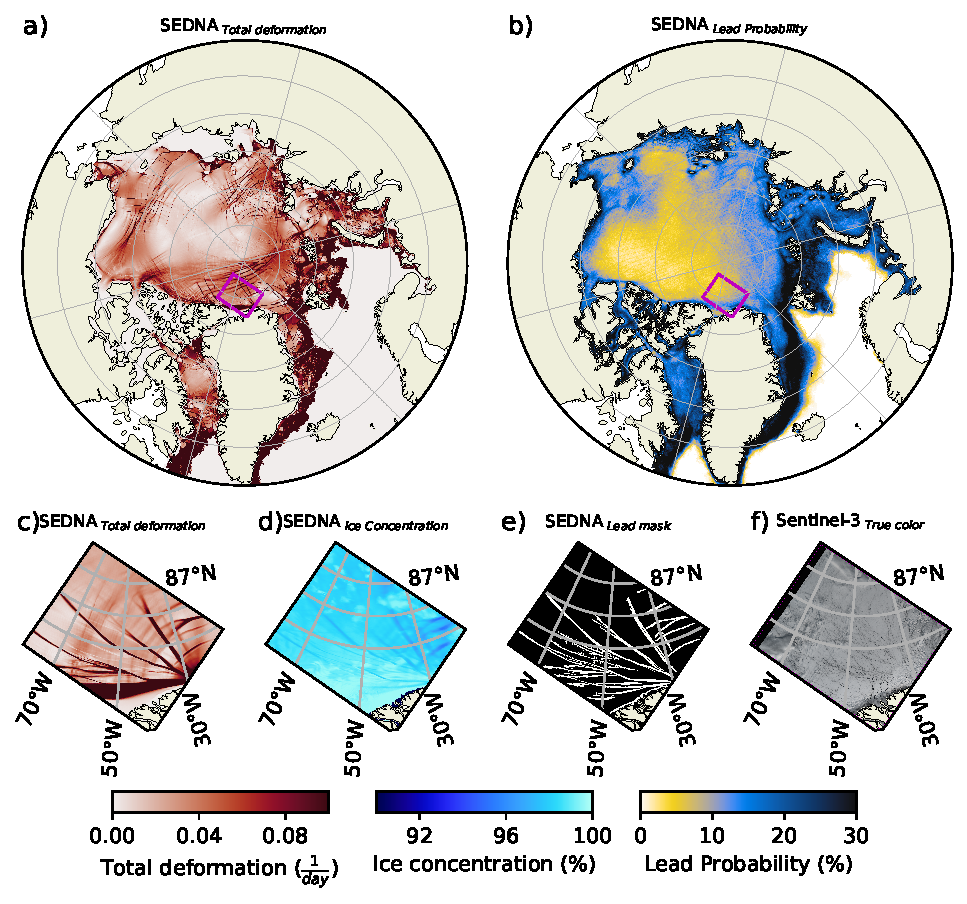
\includegraphics[width=0.95\textwidth]{./figures/Figure_1_SENTINE_SEDNA_LKF_conc_New_Color.pdf}
%DIFDELCMD <     %%%
\DIFdelendFL \DIFaddbeginFL 
\includegraphics[width=0.95\textwidth]{./Figures/Figure_1_SENTINE_SEDNA_LKF_conc_New_Color.pdf}
    \DIFaddendFL \caption{a) Snapshot of total deformation for the 21st of April 2014 from SEDNA. b) Mean lead probability for daily snapshots of leads identified between 2011 and 2015 from SEDNA. c) True color image from Sentinel 3 on the 12th of April 2022 for the magenta area in panel a. d) Snapshot of the ice concentration from SEDNA on the 21st of April 2014. e) Total deformation to identify leads and f) identified mask of leads on the 21st of April 2014 in SEDNA.}
    \label{fig:fig1}
\end{figure}

Accurate representations of leads \DIFdelbegin \DIFdel{require }\DIFdelend \DIFaddbegin \DIFadd{are captured in }\DIFaddend models with horizontal resolutions \DIFdelbegin \DIFdel{in the order }\DIFdelend of a few kilometers \citep{Bouchat_sea_ice_rheology_2022, Wang_leads_2016}\DIFdelbegin \DIFdel{; }\DIFdelend \DIFaddbegin \DIFadd{, }\DIFaddend however, to \DIFdelbegin \DIFdel{adequately resolve the localized nature of }\DIFdelend \DIFaddbegin \DIFadd{resolve localized }\DIFaddend freshwater and heat fluxes \DIFdelbegin \DIFdel{across leads, higher horizontal resolutions in the subkilometer range }\DIFdelend \DIFaddbegin \DIFadd{within leads, subkilometer resolutions }\DIFaddend are needed. \DIFdelbegin \DIFdel{To overcome this , here we analyse model }\DIFdelend \DIFaddbegin \DIFadd{We address this by analyzing }\DIFaddend outputs from the \DIFaddbegin \DIFadd{SEDNA }\DIFaddend ocean-sea ice model\DIFdelbegin \DIFdel{SEDNA, with a }\DIFdelend \DIFaddbegin \DIFadd{, which has an average Arctic }\DIFaddend resolution of $\sim 800m$\DIFdelbegin \DIFdel{on average across the Arctic capable }\DIFdelend \DIFaddbegin \DIFadd{, sufficient }\DIFaddend to capture the \DIFdelbegin \DIFdel{observational }\DIFdelend \DIFaddbegin \DIFadd{observed }\DIFaddend lead width distribution ($>1km$; \citealp{Wernecke_Lead_2015}). 
A snapshot of the total deformation is shown in figure \ref{fig:fig1}a, where regions with locally high deformation values are identified as leads (See methods\DIFdelbegin \DIFdel{for the definition of sea ice total deformation}\DIFdelend ; \citealp{Hutter_identification_2019, kwok_deformation_2001,Ruffieux_pack_lead_1995}). \DIFdelbegin \DIFdel{Zooming into the magenta box }\DIFdelend \DIFaddbegin \DIFadd{Upon closer examination of the area }\DIFaddend north of Greenland \DIFdelbegin \DIFdel{, }\DIFdelend \DIFaddbegin \DIFadd{(}\DIFaddend panels c, d, and e\DIFdelbegin \DIFdel{of figure \ref{fig:fig1}}\DIFdelend \DIFaddbegin \DIFadd{)}\DIFaddend , show that regions of high deformation match those with lower ice concentration and the identified lead mask. 
\DIFdelbegin \DIFdel{Note that the sea ice concentration in the identified }\DIFdelend \DIFaddbegin \DIFadd{Identified }\DIFaddend leads shown in figure \ref{fig:fig1}e using the lead identification algorithm proposed by \citet{Hutter_identification_2019} \DIFdelbegin \DIFdel{remains }\DIFdelend \DIFaddbegin \DIFadd{retain ice concentrations }\DIFaddend higher than 90\%\DIFdelbegin \DIFdel{concentration}\DIFdelend ; this is a consequence of continuous nature of the sea ice model and the daily averaged output that smooths the presence of leads in the fields. 
Despite the high sea ice concentration, SEDNA \DIFdelbegin \DIFdel{is capable to resolve intensified }\DIFdelend \DIFaddbegin \DIFadd{captures }\DIFaddend localized sea ice deformation. Furthermore, panels e and f reveal similarities between a typical spatial pattern of observed leads on the 12th of April 2022 from a true color satellite image and the lead mask from SEDNA for the 21st of April 2014.

The climatology of the lead probability, i.e. the likelihood of a leads occurring for any given day, is shown in figure \ref{fig:fig1}b. The mean probability of leads averaged over the Arctic is $\sim 19\%$ in SEDNA, comparable to \DIFdelbegin \DIFdel{observations using RADARSAT Geophysical Processor System and Thermal-Infrared Satellite Imagery }\DIFdelend \DIFaddbegin \DIFadd{previous observations }\DIFaddend \citep{Wernecke_Lead_2015,Willmes_leads_currents_2023}. Although observations use different identification methods compared to the one implemented in SEDNA \citep{Hutter_identification_2019}, there is resemblance between \DIFdelbegin \DIFdel{the spatial patterns of }\DIFdelend SEDNA and observations (Fig. \ref{fig:S_fig1}). We observe higher lead probability over the shelves, along bathymetric features, and in regions with large kinetic energy (Fig. \ref{fig:S_fig1}). SEDNA reproduces the \DIFdelbegin \DIFdel{patterns }\DIFdelend \DIFaddbegin \DIFadd{overall spatial patterns of lead probability }\DIFaddend observed in the Arctic\DIFdelbegin \DIFdel{shelves, the Greenland Sea, Barents Sea, Kara Sea, Laptev Sea, and hotspots in the Chukchi Sea, but the pattern in the Beaufort Seain observations is not fully captured in SEDNA}\DIFdelend \DIFaddbegin \DIFadd{, except for the Beaufort Sea}\DIFaddend . Regardless, the similarities between the observations and the model lead probability give us confidence to quantify for the first time the impact of leads in the surface buoyancy of the Arctic Ocean.

Figure \ref{fig:fig2}a and b show two snapshots of the buoyancy flux at the ocean surface. A negative buoyancy flux \DIFdelbegin \DIFdel{in winter results mainly }\DIFdelend \DIFaddbegin \DIFadd{results }\DIFaddend from sea ice refreezing and brine rejection, while \DIFdelbegin \DIFdel{, in summer, }\DIFdelend a positive buoyancy flux is associated with sea ice melting and freshening of the Arctic surface. Inside the ice covered region (magenta contour) in figure \ref{fig:fig2}, the fluxes are spatially homogeneous, except for the marginal ice zone and within the leads, where the buoyancy fluxes are larger. The area-weighted buoyancy flux across the ice covered Arctic (15\% - 100\% ice concentration) within the leads is $-2.2\times 10^{-8} m^2/s^3$ and $7.2\times 10^{-8} m^2/s^3$ for each date, compared to the $-2.4\times 10^{-8} m^2/s^3$ and $5.7\times 10^{-8} m^2/s^3$ excluding the leads. In other words, on the 1st of January (winter), the total fluxes within the leads and those outside of the leads are comparable. However, on the 25th of June (summer), the area weighted fluxes in the leads can be up to 30\% larger than those over the ice cover region \DIFdelbegin \DIFdel{without considering }\DIFdelend \DIFaddbegin \DIFadd{excluding }\DIFaddend leads.

\begin{figure}
    \centering
    \DIFdelbeginFL %DIFDELCMD < 
\includegraphics[width=1\textwidth]{./figures/Figure_2_buoyancy_flux_maps_vertical_V2_15p.pdf}
%DIFDELCMD <     %%%
\DIFdelendFL \DIFaddbeginFL 
\includegraphics[width=1\textwidth]{./Figures/Figure_2_buoyancy_flux_maps_vertical_V2_15p.pdf}
    \DIFaddendFL \caption{Maps of buoyancy flux and transects for the 1st of January and 25th of June 2014. a) Map of buoyancy flux on the 1st of January 2014. 
    Transect on the 1st of January 2014 of c) ice thickness, e) downward heat flux, g) minus freshwater flux, and i) buoyancy flux (heat flux minus freshwater flux). b) Map of buoyancy flux on the 25th of June 2014. Transect on the 25th of June 2014 of d) ice thickness, f) downward heat flux, h) minus freshwater flux, and j) buoyancy flux. Note that positive buoyancy fluxes correspond to buoyancy loss, while negative buoyancy fluxes correspond to buoyancy gain by the ocean. The transect location and orientation changes between the winter and summer dates. Magenta contour in panels a and b correspond to the 15\% concentration contour of sea ice. Vertical blue bars shows the mask of leads in the transect.}
    \label{fig:fig2}
\end{figure}

\DIFdelbegin \DIFdel{Two transects across the Beaufort Gyre are shown in figure \ref{fig:fig2} for the 1st of January 2014 and 25th of June 2014.
}\DIFdelend Examining the transect on the 1st of January 2014, we \DIFdelbegin \DIFdel{notice that along the transect we }\DIFdelend detect two leads (vertical blue bars) \DIFdelbegin \DIFdel{. Within these detected leads there is }\DIFdelend \DIFaddbegin \DIFadd{with }\DIFaddend a significant decrease in sea ice thickness of $\sim 25cm$, suggesting an opening of the sea ice cover (Fig.\ref{fig:fig2} c).
\DIFdelbegin \DIFdel{Along this transect there is an overall }\DIFdelend \DIFaddbegin \DIFadd{This transect exhibits }\DIFaddend small heat flux at the ocean surface and within the identified leads (Fig.\ref{fig:fig2} e), \DIFdelbegin \DIFdel{since }\DIFdelend \DIFaddbegin \DIFadd{because }\DIFaddend the ocean surface is at freezing point \DIFdelbegin \DIFdel{. Thus, the extra }\DIFdelend \DIFaddbegin \DIFadd{and the }\DIFaddend heat exchanged with the atmosphere is used to form sea ice instead of further cooling the ocean\DIFdelbegin \DIFdel{, resulting in a heat flux close to zero at the ocean surface.
In contrast, the }\DIFdelend \DIFaddbegin \DIFadd{.
The }\DIFaddend freshwater flux (Fig.\ref{fig:fig2}g) exhibits two prominent positive peaks, located within the identified leads. Both \DIFdelbegin \DIFdel{of these }\DIFdelend peaks are twice the magnitude of the fluxes \DIFdelbegin \DIFdel{where no leadswere identified, since there is }\DIFdelend \DIFaddbegin \DIFadd{outside the leads, thus, highlighting }\DIFaddend enhanced sea ice growth and brine rejection within the leads. 
The buoyancy flux is negative for this snapshot where the largest buoyancy loss occurs within the leads (Fig.\ref{fig:fig2} i).
On the 25th of June (Fig.\ref{fig:fig2}d), we detect several leads, but only some show a decrease of the sea ice thickness of more than $1m$ (Fig.\ref{fig:fig2} h). Leads with a sea ice thickness decrease also experience an increase in heat fluxes, reaching up to $\sim 25 W/m^2$ (Fig.\ref{fig:fig2}f) and a local decrease of the freshwater flux, indicating a freshening of the surface due to sea ice melt. This change is captured by the positive buoyancy flux, decreasing the density at the surface (Fig.\ref{fig:fig2}j).
\DIFdelbegin \DIFdel{Note that some peaks in the buoyancy flux align with the edge of the detected leads, potentially due to the enhanced refreezing or melting that occurs at the edge of the lead or the advection of the lead after it is formed. 
}\DIFdelend Of all the identified leads, some exhibit significant fluxes at the ocean surface, while others have little to no imprint in the thickness and fluxes. \DIFdelbegin \DIFdel{Detected leads  without changes in the thickness or ocean surface fluxes }\DIFdelend \DIFaddbegin \DIFadd{The latter ones }\DIFaddend may be explained by the timing of the sea ice break up, where \DIFdelbegin \DIFdel{later }\DIFdelend \DIFaddbegin \DIFadd{subsequent }\DIFaddend snapshots show an increase of fluxes at the location of these identified leads (not shown). Alternatively, previous studies have shown that leads generated through shear have a limited flux exchange with the atmosphere, but may still enhance fluxes in the ocean \DIFdelbegin \DIFdel{interior }\DIFdelend due to isopycnal upwelling or downwelling forced by the atmosphere-ocean stress within the leads \citep{Bourgault_flux_lkf_2020}.

Similar to observations, we identify fluxes that are larger within the leads than outside of them for these summer and winter days. \DIFdelbegin \DIFdel{The contribution of the freshwater flux to the total buoyancy flux, attributable to melting and freezing, is significantly larger than the heat flux contribution associated within the leads. }\DIFdelend In the next section, we explore the spatially averaged contribution of leads to the surface the buoyancy fluxes and the integrated influence on the water mass transformation across the Arctic Basin during 2014. 

\section{\DIFdelbegin \DIFdel{Mean }\DIFdelend \DIFaddbegin \DIFadd{Integrated }\DIFaddend contribution of \DIFdelbegin \DIFdel{the }\DIFdelend leads to the \DIFdelbegin \DIFdel{surface }\DIFdelend Arctic buoyancy}\label{sec3}

The ice covered Arctic experiences two main dynamical sea ice regimes, the marginal ice zone (MIZ; 15-80\% sea ice concentration) and \DIFaddbegin \DIFadd{the }\DIFaddend ice pack (80-100\% sea ice concentration). Thus, the following analysis are conducted separately for four distinct masks representing regions with leads and regions excluding leads for the MIZ and the ice pack. The averaged percentage area extent of these distinct masks during 2014 is as follows: 6\% for the MIZ, 72\% for the ice pack, 6\% for the leads in the MIZ, and 16\% for the leads in the ice pack. On average, the area extent covered by leads is $\sim 22\%$ of the total sea ice covered Arctic, consistent with previous model assessments \citep{Wang_leads_2016}. 
The extent of each mask exhibits a seasonal cycle (Fig. \ref{fig:fig3}a). From winter (December, January, and February) to  summer (June, July, and August), the percentage of the ice pack extent decreases from approximately $80\%$ to $60\%$, while the extent of the MIZ increases from $2\%$ to approximately $13\%$. 
On one hand, the percentage of the \DIFdelbegin \DIFdel{leads extent in the ice pack }\DIFdelend \DIFaddbegin \DIFadd{ice pack leads extent }\DIFaddend peaks in winter at \DIFdelbegin \DIFdel{almost }\DIFdelend 16\% \DIFdelbegin \DIFdel{of the total surface covered by ice, with }\DIFdelend \DIFaddbegin \DIFadd{and decreases to }\DIFaddend a minimum extent of 13\% in summer. On the other hand, the \DIFdelbegin \DIFdel{contribution of the leads in the MIZ covers up to 13\% of the total ice cover Arctic in summer, and around 2\% in winter. Overall the extend of leads in the MIZ is comparable to the MIZ extentexcluding the leads}\DIFdelend \DIFaddbegin \DIFadd{extent of the MIZ leads covers 2\% in winter and around 13\% in summer, approximately the same as the MIZ extent}\DIFaddend . 

The contribution of the \DIFaddbegin \DIFadd{total }\DIFaddend buoyancy flux occurring within the leads and ice covered regions \DIFdelbegin \DIFdel{excluding leads }\DIFdelend are quantified by weighting the buoyancy flux of each of the sea ice cover masks by the total ice covered area (Fig. \ref{fig:fig3}b\DIFdelbegin \DIFdel{), where }\DIFdelend \DIFaddbegin \DIFadd{; note that }\DIFaddend the extent of each \DIFdelbegin \DIFdel{ice cover }\DIFdelend mask evolves in time\DIFdelbegin \DIFdel{. When excluding the contribution within the leads, the }\DIFdelend \DIFaddbegin \DIFadd{). The }\DIFaddend mean buoyancy flux under the ice pack \DIFdelbegin \DIFdel{excluding leads }\DIFdelend in winter (December-February) and summer (June-August) is \DIFdelbegin \DIFdel{-1.8$\times10^{-8} m^2/s^3$  and 2.2$\times10^{-8} m^2/s^3$}\DIFdelend \DIFaddbegin \DIFadd{$-1.8 \times10^{-8} m^2/s^3$  and $2.2 \times10^{-8} m^2/s^3$}\DIFaddend , respectively. The buoyancy flux underneath the ice pack changes sign during the seasonal cycle, suggesting a shift from ice formation in winter to ice melting in summer. Note that in the ice pack, the haline component of the buoyancy flux determines the buoyancy flux. Meanwhile, the mean buoyancy flux in the MIZ \DIFdelbegin \DIFdel{(excluding the leads) }\DIFdelend increases from a negligible \DIFdelbegin \DIFdel{0.02$\times10^{-8}m^2/s^3$ }\DIFdelend \DIFaddbegin \DIFadd{$0.02 \times10^{-8}m^2/s^3$ }\DIFaddend in winter to \DIFdelbegin \DIFdel{0.9$\times10^{-8}m^2/s^3$ }\DIFdelend \DIFaddbegin \DIFadd{$0.9 \times10^{-8}m^2/s^3$ }\DIFaddend in summer. The MIZ has predominantly a positive buoyancy flux suggesting preferential melting over the year (except for autumn), and \DIFdelbegin \DIFdel{both thermal and haline component of }\DIFdelend \DIFaddbegin \DIFadd{the haline component also determines }\DIFaddend the buoyancy flux \DIFdelbegin \DIFdel{play a role in determining the buoyancy flux.}\DIFdelend \DIFaddbegin \DIFadd{(See Fig.\ref{fig:S_fig2}). }\DIFaddend In both the MIZ leads and the ice pack leads, the buoyancy flux follow the same seasonality \DIFdelbegin \DIFdel{as the fluxes in the MIZ and the pack }\DIFdelend \DIFaddbegin \DIFadd{of the fluxes }\DIFaddend outside of the leads. Winter values are \DIFdelbegin \DIFdel{-0.3$\times10^{-8}m^2/s^3$ and -0.01$\times10^{-8}m^2/s^3$}\DIFdelend \DIFaddbegin \DIFadd{$-0.3 \times10^{-8}m^2/s^3$ and $-0.01 \times10^{-8}m^2/s^3$}\DIFaddend , while summer values reach \DIFdelbegin \DIFdel{0.6$\times10^{-8}m^2/s^3$ and 0.9$\times10^{-8}m^2/s^3$ }\DIFdelend \DIFaddbegin \DIFadd{$0.6 \times10^{-8}m^2/s^3$ and $0.9 \times10^{-8}m^2/s^3$ }\DIFaddend for the contribution of the leads in the ice pack and the MIZ, respectively.
\DIFdelbegin \DIFdel{Comparing these fluxes weighted by the total ice covered area allows us to quantify their percentage contribution by region. 
In other words, buoyancy fluxes within the leads accounts for 15-30\% of those underneath the ice pack, while in the MIZ leads, the buoyancy fluxes are comparable to those underneath the MIZ. 
}\DIFdelend Overall, leads explain between 20\DIFaddbegin \DIFadd{\% }\DIFaddend to 45\DIFdelbegin \DIFdel{percent }\DIFdelend \DIFaddbegin \DIFadd{\% }\DIFaddend of the ice covered buoyancy fluxes (red dashed line in Fig \ref{fig:fig3}b)\DIFdelbegin \DIFdel{. This is despite the fact that the }\DIFdelend \DIFaddbegin \DIFadd{, more than the area }\DIFaddend extent of all leads \DIFaddbegin \DIFadd{that }\DIFaddend ranges from 18\% in winter to 26\% in summer\DIFdelbegin \DIFdel{of the ice covered extend}\DIFdelend . Therefore, \DIFdelbegin \DIFdel{it suggests that }\DIFdelend fluxes are larger within the leads relative to \DIFdelbegin \DIFdel{there }\DIFdelend \DIFaddbegin \DIFadd{their area }\DIFaddend extent. 

\DIFdelbegin \DIFdel{To further quantify this, the }\DIFdelend \DIFaddbegin \DIFadd{The }\DIFaddend area weighted buoyancy fluxes by each region \DIFdelbegin \DIFdel{is shown in figure \ref{fig:fig3}c. Buoyancy fluxes per unit of area exhibit two main different responses when comparing between the leads, and the MIZ and ice pack: i) winter leads in the MIZ and ii) summer leads in the ice pack.
%DIF < Winter leads in the MIZ and the summer leads in the ice pack exhibit distinct  compared to those in the MIZ and ice pack, respectively. 
First, the mean winter }\DIFdelend \DIFaddbegin \DIFadd{(Fig. \ref{fig:fig3}c) highlights the time periods in which fluxes are distinct within leads and those underneath the surrounding ice cover.
During winter, the }\DIFaddend area weighted buoyancy flux of the \DIFdelbegin \DIFdel{leads in the MIZ is 
}\DIFdelend \DIFaddbegin \DIFadd{MIZ leads is negative (}\DIFaddend -0.8 $\times10^{-8} m^2/s^3$\DIFdelbegin \DIFdel{, a negative buoyancy flux in winter within the leads }\DIFdelend \DIFaddbegin \DIFadd{), }\DIFaddend compared to a positive \DIFdelbegin \DIFdel{in }\DIFdelend \DIFaddbegin \DIFadd{one }\DIFaddend outside the leads (1.5 $\times10^{-8} m^2/s^3$). \DIFdelbegin \DIFdel{This suggests that within the leads there is }\DIFdelend \DIFaddbegin \DIFadd{Thus, in winter leads are }\DIFaddend re-freezing \DIFaddbegin \DIFadd{ice, }\DIFaddend while underneath the ice-covered MIZ \DIFdelbegin \DIFdel{there is primarily melting.  This is consistent with previous results that show more freezing occurs within leads in winter \mbox{%DIFAUXCMD
\citep{Boutin_rheology_2023}}\hskip0pt%DIFAUXCMD
. Second, the mean summer }\DIFdelend \DIFaddbegin \DIFadd{ice is melting.  During summer, the }\DIFaddend area weighted buoyancy flux within the \DIFdelbegin \DIFdel{leads in the ice pack is 4.4$\times10^{-8} m^2/s^3$}\DIFdelend \DIFaddbegin \DIFadd{ice pack leads is $4.4 \times10^{-8} m^2/s^3$}\DIFaddend , approximately 20\% more \DIFdelbegin \DIFdel{buoyancy flux in summer compared to }\DIFdelend \DIFaddbegin \DIFadd{than the buoyancy flux underneath }\DIFaddend the ice pack (\DIFdelbegin \DIFdel{3.6$\times10^{-7} m^2/s^3$ per $km^2$}\DIFdelend \DIFaddbegin \DIFadd{$3.6 \times10^{-8} m^2/s^3$}\DIFaddend ), indicating enhanced melting within the ice pack leads. 

\begin{figure}
    \centering
    \DIFdelbeginFL %DIFDELCMD < 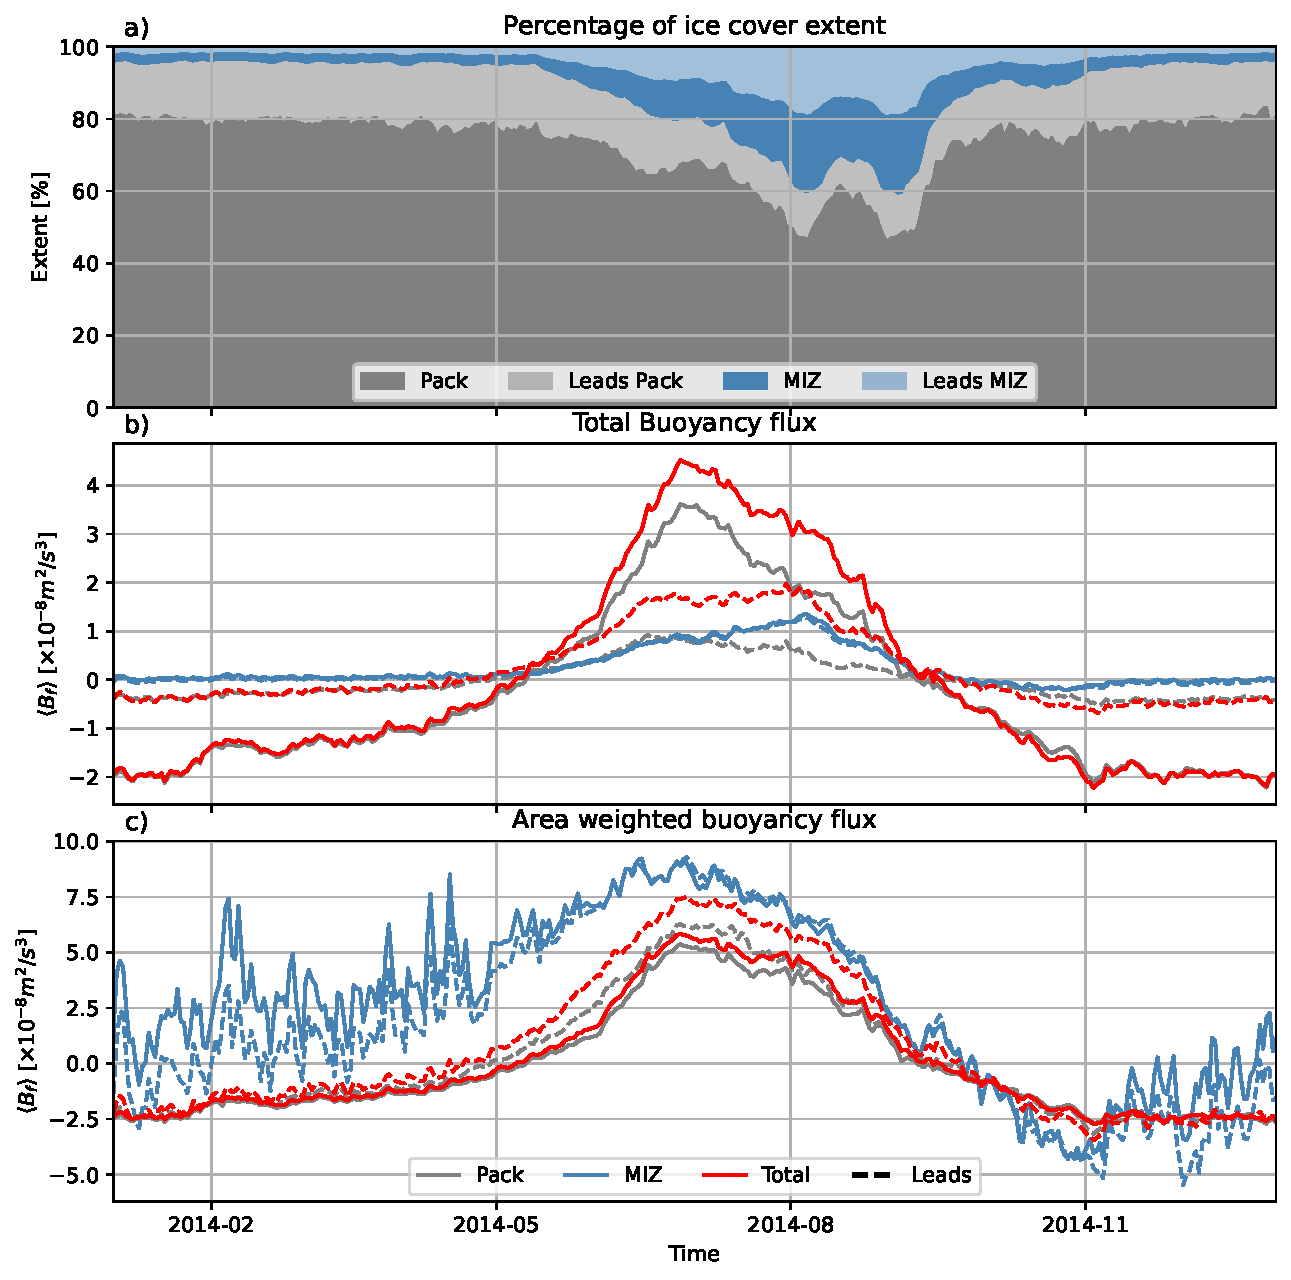
\includegraphics[width=1\textwidth]{./figures/Figure_3_buoyancy_flux_ts_full.pdf}
%DIFDELCMD <     %%%
\DIFdelendFL \DIFaddbeginFL 
\includegraphics[width=1\textwidth]{./Figures/Figure_3_buoyancy_flux_ts_full.pdf}
    \DIFaddendFL \caption{Time-series during 2014 of a) the percentage of ice cover extent, \DIFdelbeginFL \DIFdelFL{and }\DIFdelendFL b) the \DIFdelbeginFL \DIFdelFL{area-weighted }\DIFdelendFL \DIFaddbeginFL \DIFaddFL{total }\DIFaddendFL buoyancy fluxes for the \DIFaddbeginFL \DIFaddFL{total }\DIFaddendFL ice \DIFaddbeginFL \DIFaddFL{covered, the ice }\DIFaddendFL pack, the MIZ, and the leads in the ice pack and in the MIZ\DIFaddbeginFL \DIFaddFL{, and c) the area-weighted buoyancy flux}\DIFaddendFL . The MIZ is defined between ice concentration of 15-80\%, \DIFdelbeginFL \DIFdelFL{and }\DIFdelendFL the ice pack is defined where ice concentration $>80\%$\DIFaddbeginFL \DIFaddFL{, and the total ice covered is defined as the sum of the MIZ and ice pack}\DIFaddendFL .}
    \label{fig:fig3}
\end{figure}

The role and impact leads have on the surface water masses of the Arctic can be quantified by using the surface water mass transformation framework (WMT; see methods section; \citealp{Walin_WMT_1982}). This approach provides information on the transport of water through the surface density contours due to surface buoyancy forcing that results in the formation of lighter or denser water at the surface. Thus, the WMT relates the surface buoyancy forcing and the surface density field to the properties of the ocean interior. 
In figure \ref{fig:fig4}a, the averaged WMT during 2014 is shown for the total ice covered Arctic, the ice pack, the MIZ, and the parts of these regions covered by leads. The definitions of the water masses depicted in figure \ref{fig:fig4}a are taken loosely from those proposed by \DIFdelbegin \DIFdel{\mbox{%DIFAUXCMD
\citealt{Pemberton_WMT_2015, Lansard_water_mass_2012}}\hskip0pt%DIFAUXCMD
}\DIFdelend \DIFaddbegin \DIFadd{\mbox{%DIFAUXCMD
\citealt{Pemberton_WMT_2015} }\hskip0pt%DIFAUXCMD
and \mbox{%DIFAUXCMD
\citealt{Lansard_water_mass_2012}}\hskip0pt%DIFAUXCMD
}\DIFaddend .
The yearly mean WMT in the ice pack is characterized by a broad region of strong positive transformation (losing buoyancy) corresponding approximately to the halocline polar surface water ($PSW_{H}$; $24.4 kg/m^3 < \rho < 27.4 kg/m^3$) reaching a maximum of $\sim 1.8 Sv$\DIFaddbegin \DIFadd{, consistent with previous estimates of the surface Arctic WMT \mbox{%DIFAUXCMD
\citep{Pemberton_WMT_2015}}\hskip0pt%DIFAUXCMD
}\DIFaddend .
The yearly mean WMT in the ice pack leads also features a positive peak within the $PSW_{H}$ reaching up to $0.4 Sv$. On average during 2014, the WMT in the ice pack leads is $\sim 20\%$ of the WMT in the ice pack (without leads). The mean MIZ WMT is mostly negative within the density range of $20 kg/m^3 < \rho < 27.5 kg/m^3$ (gaining buoyancy), reaching a minimum of $-0.4 Sv$ around $\rho = 27 kg/m^3$. The MIZ leads WMT is also negative within the same range of densities, with a minimum also of $-0.4 Sv$. Thus, the MIZ leads WMT is comparable to those in the MIZ excluding leads. 
\DIFdelbegin \DIFdel{Maps of the surface density (Fig.\ref{fig:S_fig2}) show that water mass transformation are localized geographically; the transformation of $PSW_{H}$ occurs primarily within the Eurasian basin and a smaller contribution in the Chukchi sea, the $PSW_{ML}$ ($\rho < 24.4 kg/m^3$) occurs in the Canadian basin, and the $PDW$ and $AW$ ($27.4 kg/m^3 < \rho < 27.8 kg/m^3$ and $27.8 kg/m^3 < \rho$, respectively) occurs in the Barents and Kara seas. The ice covered water mass transformation estimated from SEDNA, the addition of the WMT in the ice pack, the MIZ, and the leads, is consistent with previous estimates of the surface Arctic WMT \mbox{%DIFAUXCMD
\citep{Pemberton_WMT_2015}}\hskip0pt%DIFAUXCMD
.
}%DIFDELCMD < 

%DIFDELCMD < %%%
\DIFdelend Hovm\"oller diagrams of the seasonal cycle of the daily WMT estimates over 2014 for the ice pack, the MIZ, and leads in each of these regions are depicted in figure \ref{fig:fig4}.
The mean WMT underneath the ice pack varies from 1.1 Sv in winter and -1.0 Sv in summer, while the WMT in the leads in the ice pack is 0.2 Sv in winter and -0.26 Sv in summer. In other words, the WMT in the ice pack leads ranges from 20 to 25\% of the WMT occurring in the pack \DIFdelbegin \DIFdel{over the year }\DIFdelend (Fig. \ref{fig:fig4}d). It is interesting to note that the patterns of the WMT \DIFdelbegin \DIFdel{across the density range }\DIFdelend for the leads and the surrounding regions excluding leads are similar (figures \ref{fig:fig4}b and c). This suggests that there is not specific water mass that is \DIFdelbegin \DIFdel{formed }\DIFdelend \DIFaddbegin \DIFadd{transformed }\DIFaddend preferentially with the leads. Rather, our results suggests that the water masses \DIFdelbegin \DIFdel{formed }\DIFdelend \DIFaddbegin \DIFadd{transformed }\DIFaddend within the leads and outside of them have similar properties. 
\DIFdelbegin \DIFdel{In summer and winter, the }\DIFdelend \DIFaddbegin \DIFadd{The }\DIFaddend WMT in MIZ leads \DIFdelbegin \DIFdel{are comparable to }\DIFdelend \DIFaddbegin \DIFadd{and }\DIFaddend those in the MIZ WMT \DIFdelbegin \DIFdel{. In fact, }\DIFdelend \DIFaddbegin \DIFadd{have comparable magnitudes }\DIFaddend over the year \DIFdelbegin \DIFdel{the WMT are comparable in magnitude }\DIFdelend (Fig. \ref{fig:fig4} g). Similarly to the leads in the ice pack, there is no evidence that leads in the MIZ could transform preferentially \DIFdelbegin \DIFdel{some }\DIFdelend specific water masses compared to the remaining MIZ. 
Adding the contribution of the WMT in all the leads in the Arctic (those in the MIZ and the ice pack), we estimate $\sim 25\%$ of the WMT \DIFdelbegin \DIFdel{occurs in leadsduring the year. This }\DIFdelend \DIFaddbegin \DIFadd{happens in leads, and this }\DIFaddend is comparable to the \DIFdelbegin \DIFdel{mean }\DIFdelend extent of leads in the Arctic ($\sim 22\%$). 
\DIFdelbegin \DIFdel{The percentage of the WMT explained by leads vary seasonally. Around $10\%$ to $25\%$ of the full WMT occurs within leads during spring, autumn, and winter. However, in summertime the WMT in leads accounts for $\sim 45\%$ of the total WMT because the WMT in the MIZ dominates the signal and the MIZ leads transform the same volume of water as the MIZ excluding leads (See Fig. \ref{fig:S_fig3}).
}\DIFdelend 

\begin{figure}[!ht]
    \centering
    \DIFdelbeginFL %DIFDELCMD < 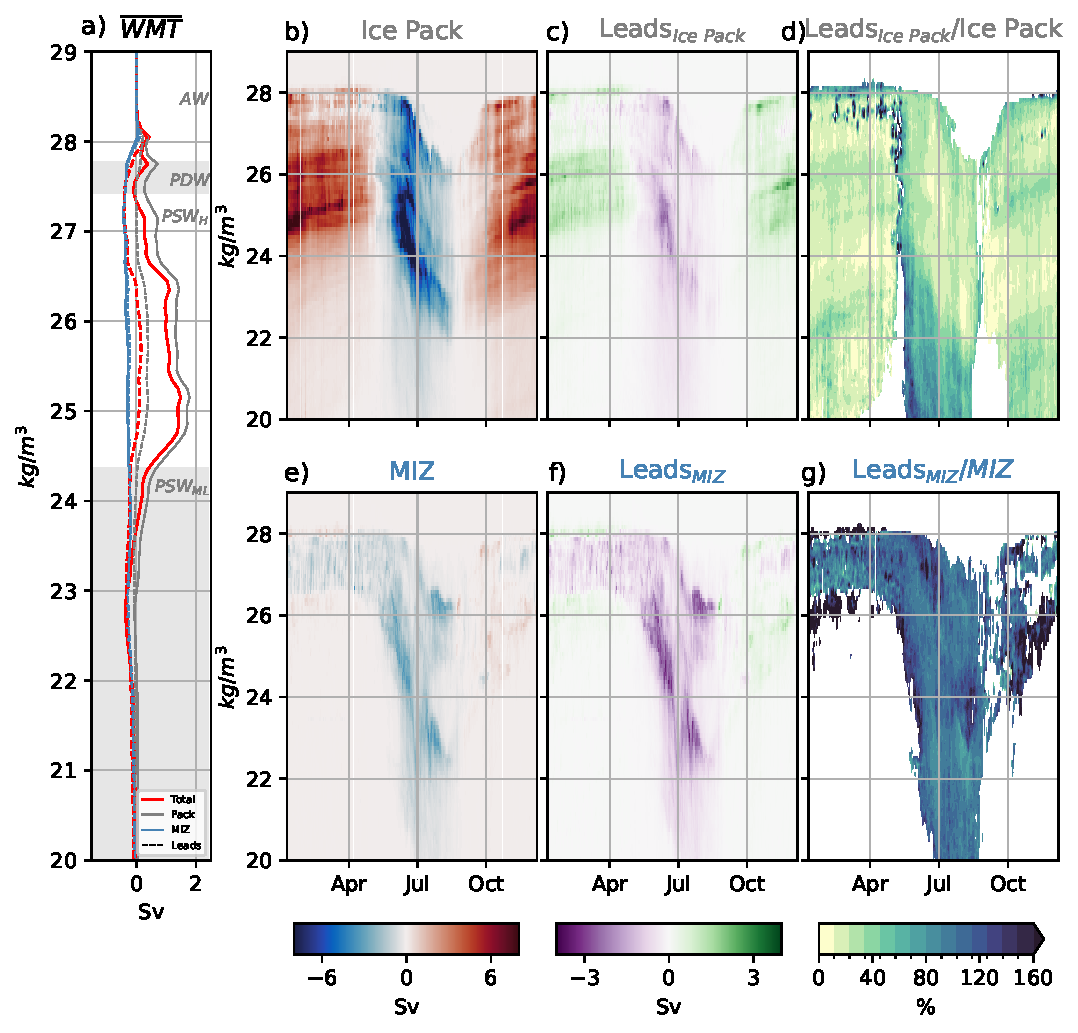
\includegraphics[width=1\textwidth]{./figures/Figure_4_water_mass_transformation_hovmoller_V2_MIZ15_80p.pdf}
%DIFDELCMD <     %%%
\DIFdelendFL \DIFaddbeginFL 
\includegraphics[width=1\textwidth]{./Figures/Figure_4_water_mass_transformation_hovmoller_V2_MIZ15_80p.pdf}
    \DIFaddendFL \caption{Mean and daily Water mass transformation over 2014. a) Mean water mass transformation over 2014 for the \DIFaddbeginFL \DIFaddFL{total }\DIFaddendFL ice \DIFaddbeginFL \DIFaddFL{covered, ice }\DIFaddendFL pack, MIZ, and leads in each region. Hovm\"oller diagram of the water mass transformation (Sv) for the b) ice pack, c) ice pack leads and d) the ratio of water mass transformation between the leads and the ice pack region.
    Panels e), f), and g) follow the same structure as panels b), c) and d), but for the MIZ, MIZ leads, and ratio between them.
    Shaded gray and white areas in panels a) represent approximately the water masses of the Arctic ocean according to \DIFdelbeginFL \DIFdelFL{\mbox{%DIFAUXCMD
\citealt{Pemberton_WMT_2015, Lansard_water_mass_2012}}\hskip0pt%DIFAUXCMD
}\DIFdelendFL \DIFaddbeginFL \DIFaddFL{\mbox{%DIFAUXCMD
\citealt{Pemberton_WMT_2015} }\hskip0pt%DIFAUXCMD
and \mbox{%DIFAUXCMD
\citealt{Lansard_water_mass_2012}}\hskip0pt%DIFAUXCMD
}\DIFaddendFL : the mixed layer polar surface water (\DIFdelbeginFL \DIFdelFL{$PSW_{ML}$; $\rho < 24.4 kg/m^3$}\DIFdelendFL \DIFaddbeginFL \DIFaddFL{$PSW_{ML};\ \rho < 24.4 kg/m^3$}\DIFaddendFL ), the halocline polar surface water (\DIFdelbeginFL \DIFdelFL{$PSW_{H}$; $24.4 kg/m^3 < \rho < 27.4 kg/m^3$}\DIFdelendFL \DIFaddbeginFL \DIFaddFL{$PSW_{H};\ 24.4 kg/m^3 < \rho < 27.4 kg/m^3$}\DIFaddendFL ), the polar deep water (\DIFdelbeginFL \DIFdelFL{$PDW$; $27.4 kg/m^3 < \rho < 27.8 kg/m^3$}\DIFdelendFL \DIFaddbeginFL \DIFaddFL{$PDW;\ 27.4 kg/m^3 < \rho < 27.8 kg/m^3$}\DIFaddendFL ), and the Atlantic water (\DIFdelbeginFL \DIFdelFL{$AW$; $27.8 kg/m^3 < \rho$}\DIFdelendFL \DIFaddbeginFL \DIFaddFL{$AW;\ 27.8 kg/m^3 < \rho$}\DIFaddendFL ).}
    \label{fig:fig4}
\end{figure}

\section{Conclusions}

\DIFdelbegin \DIFdel{Leads are ubiquitous in the sea ice covered regions. They allow exchanges between the ocean and the atmosphere and locally enhance melting and freezing of sea ice. }\DIFdelend The present study assesses the impact of leads in the ocean surface by diagnosing the buoyancy fluxes using a very high-resolution hindcast (SEDNA). The lead identification algorithm implemented in SEDNA allows us to reproduce the observed spatial distribution of leads over most regions of the Arctic, with exception of the Beaufort Sea, where the simulation underestimates the lead frequency. Likely because of the different identification algorithm, time periods, and spatial and temporal scales used in the present study and that of \citealp{Willmes_leads_currents_2023}. Despite these regional differences, SEDNA can estimate the mean lead probability, showcasing its capacity to capture the dynamics of these features.
\DIFdelbegin \DIFdel{This high resolution simulation allows us to better understand the role of leads in shaping the buoyancy fluxes of the Arctic Ocean.
}\DIFdelend 

Using SEDNA, we found that leads cover $\sim 22\%$ of the sea-ice covered Arctic, and in the ice pack, leads can contribute \DIFdelbegin \DIFdel{up to 20\% }\DIFdelend more buoyancy flux compared to the fluxes outside the leads. Despite these larger buoyancy fluxes, leads only account for approximately $\sim 25\%$ of the total surface water mass transformation in the ice covered Arctic, which is roughly equivalent to their area coverage. Thus, contrary to previous hypotheses, our findings suggest that leads have a smaller contribution to the transformation of surface water masses in the Arctic Ocean than previously thought (e.g. \citealp{Hutter_identification_2019, McPhee_LKF_2005}). While their presence can induce localized changes in the density of surface waters due to brine rejection and ice melting, 
\DIFdelbegin \DIFdel{their frequency, spatial extent and duration are not sufficient to significantly alter the water masses. It has been argued that under sea-ice cover in winter, brine rejection is not sufficient to penetrate the base of the mixed later \mbox{%DIFAUXCMD
\citep{Lenn_mixing_2022}}\hskip0pt%DIFAUXCMD
, this also appears the case for leads that are unable of imprinting a signal in the Arctic Ocean interior. For example, we noted in SEDNA that the mixed layer depth (MLD) varies underneath the ice pack leads compared to regions outside the leads, however there is no evidence of an impact in the ice cover nor a response in the surface buoyancy or change of the water mass transformation within these regions. Furthermore, the transformation }\DIFdelend \DIFaddbegin \DIFadd{the transformation }\DIFaddend of water masses in the leads have the same sign and magnitude as those underneath the surrounding ice-covered regions\DIFdelbegin \DIFdel{(excluding leads)}\DIFdelend . Thus, no evidence was found that leads impact in a distinct way the Arctic ocean water masses in SEDNA.

Here we focus on the surface forced WMT, but leads could further impact properties at the surface and interior of the ocean by enhancing mixing within leads, upwelling of isopycnals through Ekman pumping \citep{McPhee_LKF_2005}, modifying  entrainment in the mixed layer within the leads, providing a source of potential energy, and generating mixed layer instabilities due to isopycnal tilting in the vicinity of leads. \DIFdelbegin \DIFdel{A limitation of our study is the }\DIFdelend \DIFaddbegin \DIFadd{The }\DIFaddend use of a continuous sea ice model that results in leads with high ice thickness and concentrations \DIFdelbegin \DIFdel{, thus limiting }\DIFdelend \DIFaddbegin \DIFadd{limits }\DIFaddend the exchanges between the ocean and the atmosphere. \DIFdelbegin \DIFdel{In contrast}\DIFdelend \DIFaddbegin \DIFadd{Therefore}\DIFaddend , future studies using floe resolving models that allow more ``realistic leads" with direct exchanges between the ocean an the atmosphere would likely result in larger fluxes through the leads increasing their potential impact in the water mass transformation and ocean mixed layer.

Leads have an important local effect in the atmosphere and the sea-ice fluxes \citep{Lupkes_leads_2008,Marcq_flux_lead_2012, Wettlaufer_insulator_1997, Smith_polynyas_1990}, but a limited imprint on the ocean surface and interior properties. Our results suggest that the presence of leads is not the first order mechanism controlling the water mass transformation forced at the surface, thus leads have a minor impact in the stratification and surface layer dynamics of the Arctic Ocean.
Therefore, resolving and/or parameterizing leads in climate models are likely to have a negligible impact improving the \DIFdelbegin \DIFdel{well known issue within the Arctic climate modeling community of the }\DIFdelend misrepresentation of the stratification and water masses in \DIFdelbegin \DIFdel{the Arctic ocean }\DIFdelend \DIFaddbegin \DIFadd{Arctic climate models }\DIFaddend \citep{Wang_ompi_2024,Ilicak_core_2016}. Finally, the probability of leads to occur in the ice pack has been projected to increase as the Arctic sea ice transitions towards thinner, younger, and more mobile sea ice \citep{Boutin_rheology_2023, IPCC_arctic_2022}. Our analysis is only performed over one year and the future impact of more abundant leads is not represented in our simulation. Thus, dedicated studies are required to better estimate the surface buoyancy forcing within leads in the context of an evolving Arctic Ocean.  

\section{Methods}
\subsection*{Model description}

Here we employ the NEMO numerical platform (release 4.0.5; \citealp{NEMO_man}) to establish a 1/60$^\circ$ pan-Arctic ocean-sea ice configuration named SEDNA. The ocean core (NEMO-OPA) solves the primitive equations using finite differences on an Arakawa C-grid mesh, and it is coupled to the SI3 sea-ice component (NEMO-SI3; \citealp{SI3_man}). The pan-Arctic domain covers the Bering Strait on the Pacific side and extends southward to 56$^\circ$N in the Subpolar North Atlantic and to the Baltic Sea entrance. The ocean model incorporates a linear free surface, utilizes a 3rd order flux form scheme for momentum advection, and employs a 4th order Flux Corrected Transport (FCT) for tracer advection. Additionally, the sea-ice representation uses an Elasto-Visco-Plastic (EVP) rheology with a 5-categories sea ice thickness distribution and a land-fast parameterization to better simulate sea-ice behavior above shelves.

The NCAR bulk formula from \citet{Large_global_2009} is used to calculate air-sea fluxes based on the hourly ERA5 atmospheric data for near-surface variables \citep{Hersbach_ERA5_2020}. The three lateral boundaries are constrained with daily GLORYS12V1 Re-analysis data \citep{GLORYS12}. Monthly freshwater fluxes from river discharges are combined with Greenland land ice melt data \citep{HuEA_rivers_2019}. The simulation extends over seven years (2009 to 2015) and starts from rest, utilizing initial conditions based on the World Ocean Atlas 2009 temperature/salinity and mean January 2009 ice state from PIOMAS re-analysis \citep{Locarnini_data_2010, PIOMAS}. The sea surface salinity is restored to the World Ocean Atlas climatology, but it is only applied \DIFdelbegin \DIFdel{in }\DIFdelend \DIFaddbegin \DIFadd{over }\DIFaddend the ice-free ocean. Preliminary assessment against available observations and re-analyses data shows that the simulation reasonably captures key ocean and sea-ice characteristics.

\subsection*{Identification of leads}

The leads from SEDNA are identified by using the algorithm proposed by \citet{Hutter_identification_2019}. This method uses the total deformation rate defined as: 
\begin{equation}
    T_d = \left[\left(\underbrace{\frac{\partial u}{\partial x} +\frac{\partial v}{\partial y}}_{Divergence}\right)^2 + \underbrace{\left(\frac{\partial u}{\partial x} - \frac{\partial v}{\partial y}\right)^2+ \left(\frac{\partial u}{\partial y} + \frac{\partial v}{\partial x}\right)^2}_{Shear}\right]^{1/2},
\end{equation}
where $u$ and $v$ are the sea ice velocities. The deformation rate varies spatially depending on the background deformation and the sea ice properties \citep{Reiser_LKF_2020}, where the largest deformation rates occur along the boundaries of ice floes where the leads are found. Therefore, to identify the leads, the local maxima is identified using a difference of Gaussian filter (DoG filter) of the deformation rate field. After this, a binary map is created with the mask of identified lead. Note that after this step, \citet{Hutter_identification_2019} reduce the leads width to a line to then track the leads over time. Since our study focus on the ocean-atmosphere interactions, we only use the identification algorithm to produce a mask of leads during 2014 for the Arctic, thus we retain the original lead width computed from the deformation rate. Finally, the lead mask is then used to quantify and contrast the impact of leads compared to the ice covered Arctic, the ice-pack (ice concentration $> 80\%$) and the MIZ (0 - 80\% ice concentration).

\subsection*{Buoyancy flux and water mass transformation}

Heat fluxes (shortwave radiation, longwave radiation, latent heat, and sensible heat) and freshwater fluxes (evaporation, precipitation, runoff, and sea ice melt/growth) at the ocean surface result in a buoyancy forcing capable to change the density of the ocean surface. Here, the buoyancy flux is computed as:

\begin{equation}
    B_f = \underbrace{\frac{g \alpha Q_{net}}{\rho_0 C_p}}_{Net\ surface\ heat\ flux} - \underbrace{\frac{g \beta F_{net} SSS }{\rho_0}}_{Net\ surface\ freshwater\ flux},
\end{equation}

where $Q_{net}$ the net heat flux at the sea surface, $\alpha$ the thermal expansion coefficient, $SSS$ the sea surface salinity, $F_{net}$ the net fresh water flux that includes evaporation, precipitation, runoff, and freezing minus melting flux, and $\beta$ the haline contraction coefficient. With constant values of $g = 9.81 m/s^2$ and the ocean density $\rho_0 = 1026 kg/m^3$. 
Note that using this sign convention, positive values in the buoyancy forcing decrease the surface density making the ocean surface more buoyant (stable) and negative values increase the surface density. The area-weighted buoyancy ($ \left<\right>$) fluxes are computed following:

\begin{equation}
    \left<B_f (t)\right>  = \frac{\sum_x \sum_y \left( B_f(t,x,y) * Area(x,y) * Mask_{_R}(t,x,y)\right)}{\sum_x \sum_y * Area(x,y) * Mask(t,x,y)},
\end{equation}
where the $Area$ is be the area of the grid cells, and the $Mask$ is the mask of MIZ, the Pack, the MIZ leads, and the ice pack leads that vary in space and time. Note that in Figure \ref{fig:fig3}b ${equation}$ (the divisor) corresponds to the full ice covered area (including leads), while in Figure \ref{fig:fig3}c $Mask$ is equal to $Mask_{_R}$.

\citet{Nurser_WMT_1999} and  \citet{Walin_WMT_1982} proposed the water mass transformation framework that quantifies the rate at which a given water mass is made lighter (negative transformation rate) or denser (positive) due to surface fluxes. The surface water mass transformation is computed as:

\begin{equation}
    \Omega(\sigma_k) = - \frac{1}{\sigma_{k+1}-\sigma_k}\iint_AB_fdA,
\end{equation}

% \begin{equation}
%     \Omega(\sigma_k) = \underbrace{- \frac{1}{\sigma_{k+1}-\sigma_k}\iint_A\left(\frac{\alpha Q_{net}}{\rho_0 C_p}\right)dA}_{Net\ surface\ heat\ flux} + \underbrace{\frac{1}{\sigma_{k+1}-\sigma_k}\iint_A\left(\frac{\beta F_{net} SSS }{\rho_0}\right)dA}_{Net\ surface\ freshwater\ flux},
% \end{equation}

where $\sigma$ is potential density and the indices $k$ represents the density bin number. The computation was performed with 172 density bins of $0.1 kg/m^3$ within the density range of $15.15 kg/m^3$ - $32.25 kg/m^3$. The transformation rate $\Omega$ is spatially decomposed into different sea-ice masks such as the ice covered, the pack ice, the MIZ, and the leads in each of these regions. 
%By separately diagnosing the density transformation that occurs in the leads and underneath the surrounding floes, we quantify the relative importance of the leads for each of these regions. Additionally, this framework accounts for the area changes of the ice cover during the seasonal cycle, and excludes open ocean regions.

\backmatter

\bmhead{Open Source}

The SEDNA model configuration are described and publicly available at \url{https://zenodo.org/records/7656924}.
All analyses and figures in this manuscript are reproducible via Jupyter notebooks and instructions can be found in the GitHub repository \texttt{Leads\_Arctic\_ocean} (\url{https://github.com/josuemtzmo/Leads_Arctic_ocean}).

\bmhead{Acknowledgements}

We acknowledge funding from the ANR ImMEDIAT project (ANR-18-CE01-0010) and the MEDLEY project funded by the program JPI Ocean/JPI Climate (ANR-19-JPOC-0001) project. 
The idealized simulations and their analysis were performed using the HPC facilities DATARMOR of ’Pôle de Calcul Intensif pour la Mer’ at Ifremer, Brest, France. We also acknowledge PRACE for awarding us access to Joliot-Curie at GENCI\makeatletter@CEA, France, where the SEDNA simulation has been performed.

%%===========================================================================================%%
%% If you are submitting to one of the Nature Portfolio journals, using the eJP submission   %%
%% system, please include the references within the manuscript file itself. You may do this  %%
%% by copying the reference list from your .bbl file, paste it into the main manuscript .tex %%
%% file, and delete the associated \verb+\bibliography+ commands.                            %%
%%===========================================================================================%%

%% if required, the content of .bbl file can be included here once bbl is generated
%%\input sn-article.bbl


\bibliography{biblio}


\pagebreak

\begin{appendices}

\renewcommand{\thefigure}{S\arabic{figure}}

\begin{figure}
    \centering
    \DIFdelbeginFL %DIFDELCMD < 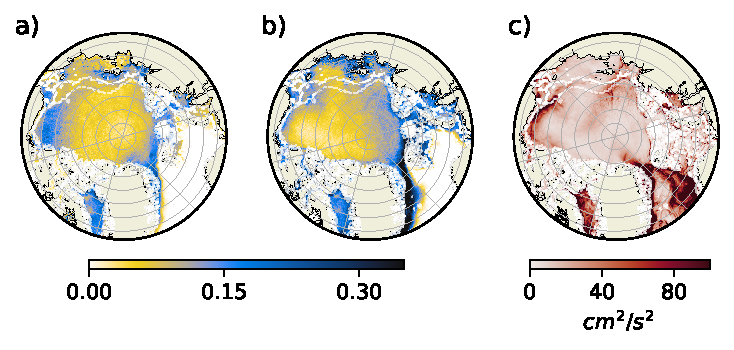
\includegraphics[width=1\textwidth]{./figures/Figure_S2_comparison_LKF_observations_KE_bathy.pdf}
%DIFDELCMD <     %%%
\DIFdelendFL \DIFaddbeginFL 
\includegraphics[width=1\textwidth]{./Figures/Figure_S1_comparison_LKF_observations_KE_bathy.pdf}
    \DIFaddendFL \caption{Comparison of winter lead frequency between a) Thermal-Infrared Satellite Imagery \citep{Willmes_leads_currents_2023} and b) SEDNA between 2011 and 2015. Panel c) shows the SEDNA mean kinetic energy between 2011 and 2015.}
    \label{fig:S_fig1}
\end{figure}

\begin{figure}
    \centering
    \DIFdelbeginFL %DIFDELCMD < 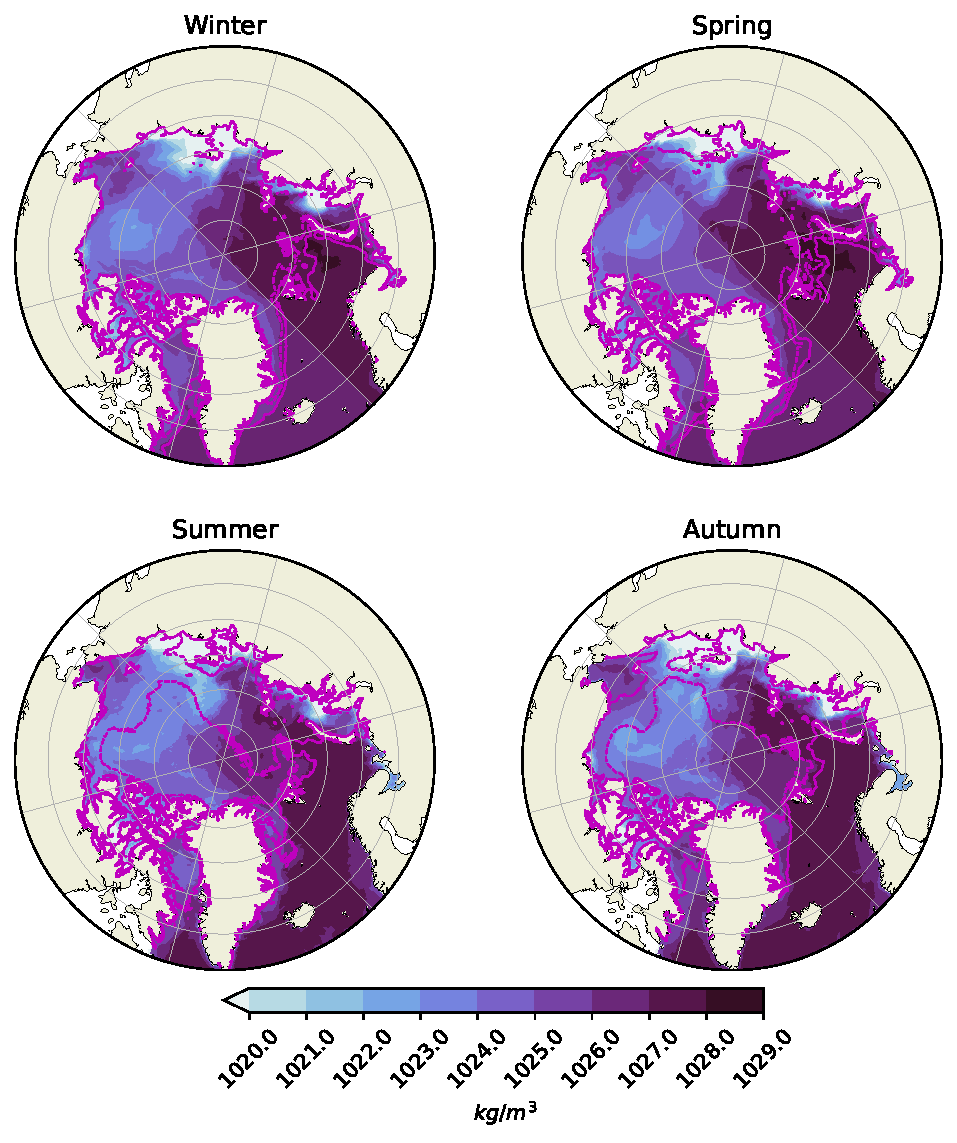
\includegraphics[width=1\textwidth]{./figures/Figure_S1_density_maps_season.pdf}
%DIFDELCMD <     %%%
\DIFdelendFL \DIFaddbeginFL 
\includegraphics[width=1\textwidth]{./Figures/Figure_S2_buoyancy_flux_components.pdf}
    \DIFaddendFL \caption{\DIFdelbeginFL \DIFdelFL{Maps }\DIFdelendFL \DIFaddbeginFL \DIFaddFL{Time-series during 2014 }\DIFaddendFL of \DIFaddbeginFL \DIFaddFL{a) }\DIFaddendFL the \DIFdelbeginFL \DIFdelFL{seasonal surface density }\DIFdelendFL \DIFaddbeginFL \DIFaddFL{freshwater component }\DIFaddendFL of \DIFdelbeginFL \DIFdelFL{SEDNA during 2014. Solid }\DIFdelendFL \DIFaddbeginFL \DIFaddFL{the buoyancy flux }\DIFaddendFL and \DIFdelbeginFL \DIFdelFL{dashed magenta contour }\DIFdelendFL \DIFaddbeginFL \DIFaddFL{b) the heat component of the buoyancy flux for the ice pack, the MIZ, and the leads }\DIFaddendFL in \DIFdelbeginFL \DIFdelFL{maps correspond to }\DIFdelendFL the \DIFdelbeginFL \DIFdelFL{15\% }\DIFdelendFL \DIFaddbeginFL \DIFaddFL{ice pack }\DIFaddendFL and \DIFdelbeginFL \DIFdelFL{80 \% }\DIFdelendFL \DIFaddbeginFL \DIFaddFL{in the MIZ. The MIZ is defined between ice }\DIFaddendFL concentration \DIFdelbeginFL \DIFdelFL{contour }\DIFdelendFL of \DIFdelbeginFL \DIFdelFL{sea }\DIFdelendFL \DIFaddbeginFL \DIFaddFL{15-80\%, and the }\DIFaddendFL ice \DIFdelbeginFL \DIFdelFL{respectively}\DIFdelendFL \DIFaddbeginFL \DIFaddFL{pack is defined where ice concentration $>80\%$}\DIFaddendFL .}
    \label{fig:S_fig2}
\end{figure}
\DIFdelbegin %DIFDELCMD < 

%DIFDELCMD < \begin{figure}
%DIFDELCMD <     \centering
%DIFDELCMD <     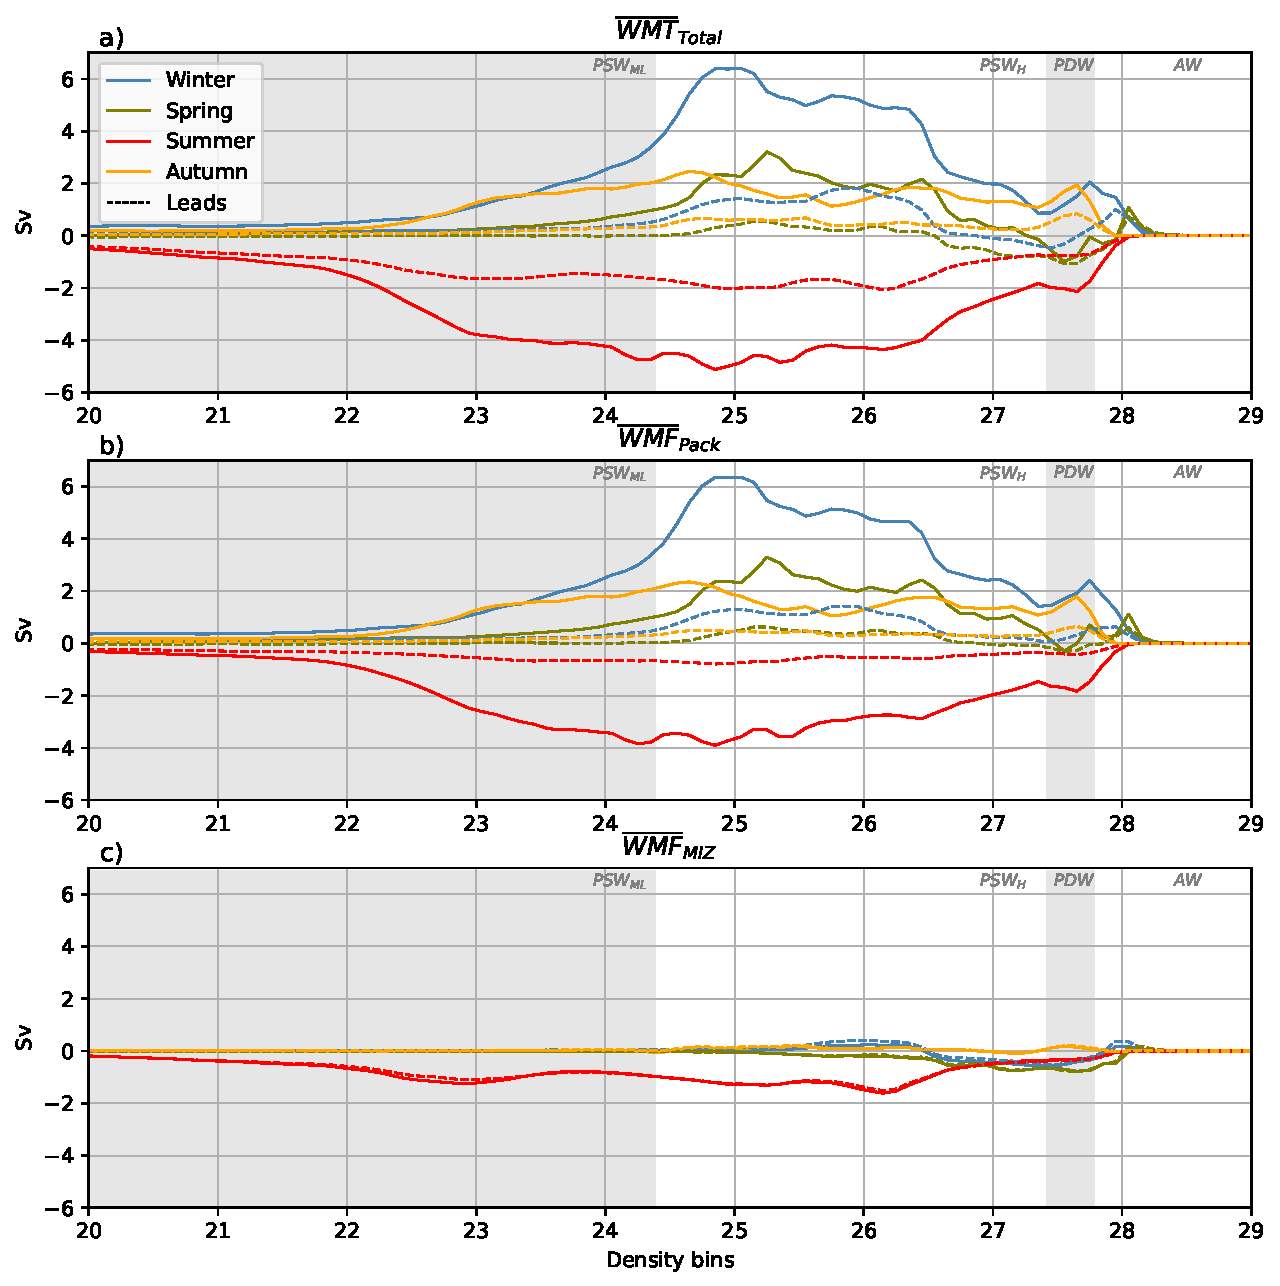
\includegraphics[width=1\textwidth]{./figures/Figure_S3_water_mass_transformation_seasonality.pdf}
%DIFDELCMD <     %%%
%DIFDELCMD < \caption{%
{%DIFAUXCMD
\DIFdelFL{Seasonal average of the water mass transformation during 2014 for a) the ice covered, b) the ice pack, and c) the MIZ. Dashed lines correspond to the WMT for the leads in each of these regions.}}
    %DIFAUXCMD
%DIFDELCMD < \label{fig:S_fig3}
%DIFDELCMD < \end{figure}
%DIFDELCMD < 

%DIFDELCMD < %%%
%DIF <  \begin{figure}
%DIF <      \centering
%DIF <      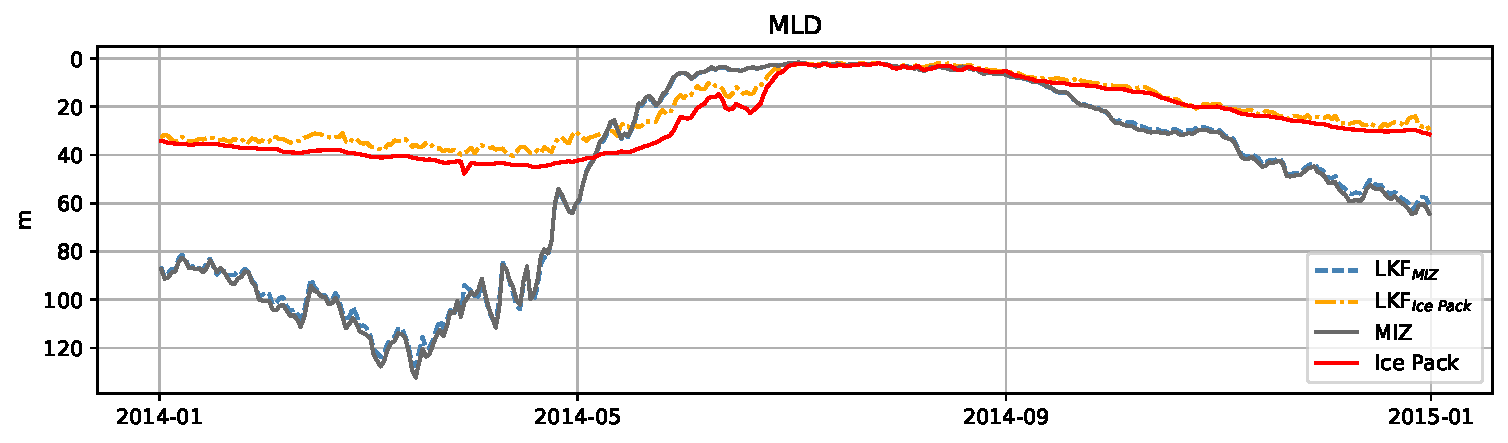
\includegraphics[width=1\textwidth]{./figures/Figure_S2_TS_MLD.pdf}
%DIF <      \caption{Time-series during 2014 of the mean mixed layer depth for linear kinematic features in the ice pack, the linear kinematic features in the marginal ice zone, the marginal ice zone (ice concentration 0-80\%), and the ice pack (ice concentration $>80\%$). The mixed layer depth is defined as the 0.1 density anomaly referenced to the first ocean model level.}
%DIF <      \label{fig:S_fig2}
%DIF <  \end{figure}
\DIFdelend 

\end{appendices}

\end{document}
